\lecture{Técnicas de múltiplo acesso}{lec_ma}

\begin{frame}
	\begin{block}{\centering\large\bfseries Parte 8}
		\centering\large\insertpart
	\end{block}
\end{frame}


\section{Introdução}

\begin{frame}
	\frametitle{Introdução}

	\begin{itemize}
	    \item Transição de um sistema de comunicação digital ponto-a-ponto para uma \textit{rede de comunicações digitais}.
	    \item Comunicação simultânea entre vários usuários.
	    \item Métodos para compartilhar o meio de acesso entre diversos usuários.
	    \item Compartilhamento de um único recurso: técnicas de \textit{contenção}.
	    \item Questões relacionadas a sincronismo entre usuários da rede.
	    \item Aplicações práticas de múltiplo acesso:
	    \begin{itemize}
		\item Transmissão \textit{full-duplex} em um meio comum.
		\item Múltiplos canais compartilhando um enlace comum de transmissão: multiplexação.
	    \end{itemize}	    
	    \item Ortogonalidade: tempo, frequência, código, espaço, etc.
	\end{itemize}			
\end{frame}

\section{Topologias de múltiplo acesso}

\begin{frame}
	\frametitle{Topologias de múltiplo acesso}

	\begin{itemize}
	    \item Topologia: configuração geométrica do meio de transmissão.
	    \item Exemplos de topologias representativas: 
	\end{itemize} \vspace{-0.2cm}
	    \begin{figure}[t]	
	    \begin{center}
		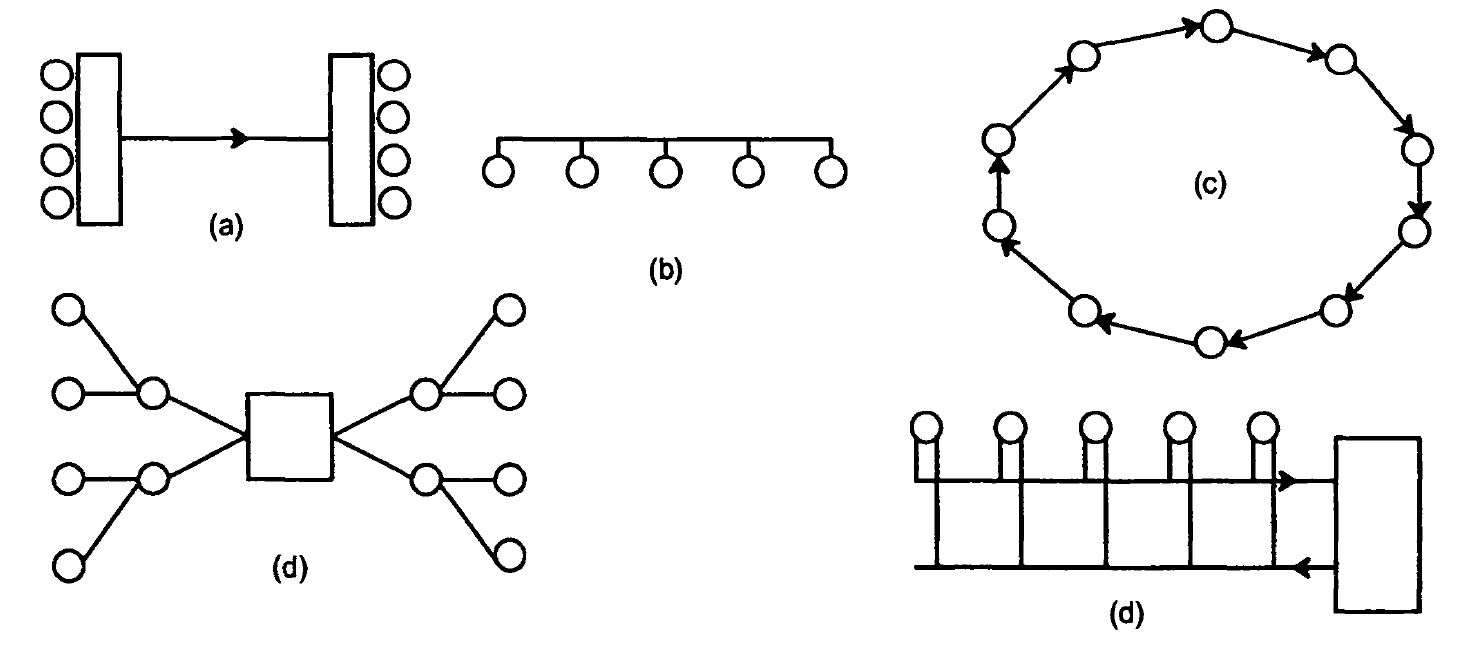
\includegraphics[width=0.75\columnwidth]{figs/ma_01}
	    \end{center}
	    \end{figure} \vspace{-0.2cm}
	    \begin{footnotesize}a) Meio unidirecional com mux/demux. b)Barramento. c) Anel. d) Árvore com nó central. e) Barramento com controle central.\end{footnotesize}
\end{frame}

\section{Técnicas de múltiplo acesso}

\begin{frame}
	\frametitle{Enlace ponto-a-ponto}

	\begin{itemize}
	 \item Conservação do tempo: a transmissão de cada amostra ocupa o canal de comunicação por somente uma fração do período de amostragem.
         \item Tempo entre amostras adjacentes fica livre para ser usado por outras fontes independentes de mensagem;
	\end{itemize}
	\begin{block}{Sistema TDM}
	    Permite a utilização conjunta de um canal de comunicação comum por uma pluralidade de fontes de mensagens independentes sem interferência mútua entre elas.
	\end{block}
	\begin{figure}
	  \begin{center}
	    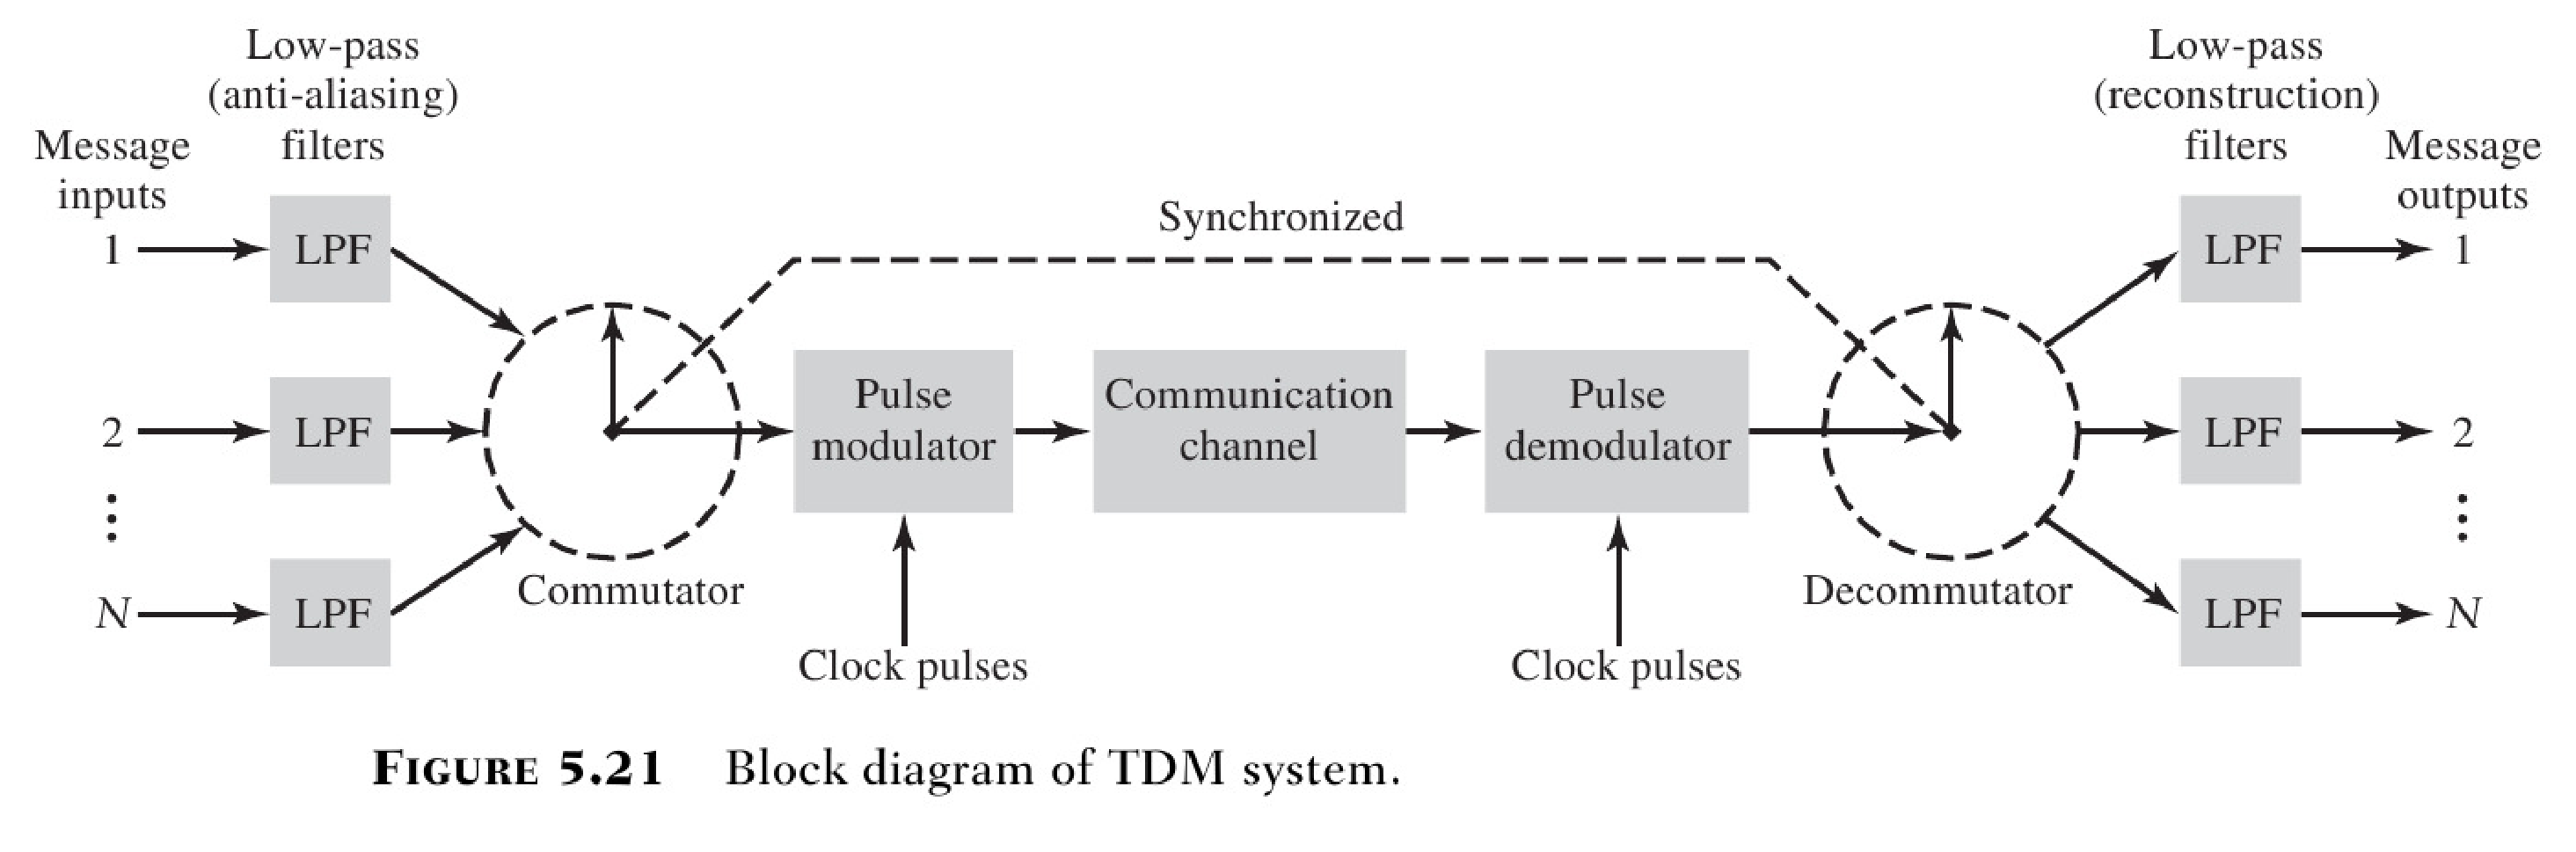
\includegraphics[width=0.9\columnwidth]{figs/fig05-21}
	  \end{center}
	\end{figure}
\end{frame}

\begin{frame}
 	\frametitle{Múltiplo acesso - FDMA}
 
	\begin{itemize}
		\item FDMA (Frequency Division Multiple Access)
		\item Caracteriza a primeira geração analógica da telefonia celular baseada em modulação FM
		\item A faixa total alocada para o sistema é dividida em canais para comunicação full-duplex
		\item Exemplo
		\begin{itemize}
			\item Banda total: 25 MHz, banda de guarda: 5 MHz
			\item Faixa para enlace direto: 800 a 812,5 MHz
			\item Faixa para enlace reverso: 817,5 a 830 MHz
			\item Canal de voz simplex: 30 kHz
			\item Total de canais de voz full-duplex: 25x103 / (2x30) = 416 canais
			\item Canal 1: direto 800,000 MHz; reverso 817,500 MHz
			\item Canal 2: direto 800,030 MHz; reverso 817,530 MHz ...
		\end{itemize}

	\end{itemize}
 \end{frame}
 
\begin{frame}
 	\frametitle{Outras técnicas de múltiplo acesso}
 
	\begin{itemize}
		\item  FDMA - utilizado nos sistemas analógicos de 1a geração
		\item Sistemas de 2$^a.$ geração baseados em TDMA e CDMA
		\vspace{0.1cm}\item TDMA – Time Division Multiple Access
		\begin{itemize}
			\item Particiona cada canal em fatias no tempo (time-slots) que são alocadas para diferentes usuários
			\item Transmissão digital da voz através de algoritmos de compressão
		\end{itemize}
		\vspace{0.1cm}\item CDMA – Code Division Multiple Access
		\begin{itemize}
			\item Associa um código secreto para cada usuário, os quais podem transmitir ao mesmo tempo e na mesma freqüência
			\item O receptor conhece o código, sendo capaz de detecter o sinal
		\end{itemize}
		\vspace{0.1cm}\item SDMA – Space Division Multiple Access
		\begin{itemize}
			\item Separação espacial dos usuários através de múltiplas antenas
		\end{itemize}

	\end{itemize}
 \end{frame}

  
 \section{Técnicas de acesso aleatório}
 
 \begin{frame}
	\frametitle{Modelo multiacesso considerado}

	\begin{itemize}
		\item Usuários:
		\begin{itemize}
			\item Os quadros chegam de forma aleatória e independente em cada usuário.
		\end{itemize}
		\item Canal:
		\begin{itemize}
			\item Toda comunicação ocorre em um único canal e não há outra forma de comunicação entre usuários.
		\end{itemize}
		\item Transmissão:
		\begin{itemize}
			\item Erros só ocorrem devido a colisões, ou seja, quando quadros chegam sobrepostos temporalmente.
		\end{itemize}
		\item Feedback:
		\begin{itemize}
			\item Os usuários são capazes de detectar colisões após o envio de quadros, desconsiderando atrasos.
		\end{itemize}
	\end{itemize}
\end{frame}

\begin{frame}
	\frametitle{Protocolos Aloha}

	\begin{itemize}
		\item Quando um usuário transmite, e não há outro usuário transmitindo ao mesmo tempo, não há colisão e o quadro é recebido com sucesso.
		\item Caso haja colisão?
		\begin{itemize}
			\item Retransmissão simples não adianta, pois o outro usuário envolvido também retransmitiria.
			\item Forma de evitar: cada usuário espera um tempo aleatório antes de retransmitir.
		\end{itemize}
		\item Protocolo Aloha:
		\begin{itemize}
			\item Desenvolvido na Universidade do Hawaii nos anos 70.
			\item Base para muitos outros protocolos de contenção.
		\end{itemize}
	\end{itemize}
\end{frame}

\begin{frame}
	\frametitle{Aloha puro}

	\begin{itemize}
		\item Usuários transmitem sempre que possuem dados.
		\item Transmissores esperam para saber se houve colisão (após o envio de toda a mensagem).
		\item Em caso de colisão, cada usuário envolvido espera um tempo aleatório e retransmite.
		\item Perguntas:
		\begin{itemize}
			\item Qual o desempenho do protocolo?
			\item Como escolher o tempo de espera?
		\end{itemize}
	\end{itemize}
\end{frame}

\begin{frame}
	\frametitle{Aloha puro}

	\begin{itemize}
		\item Os quadros são transmitidos em tempos arbitrários:
	\end{itemize}
	
	\begin{figure}[t]
		\begin{center}
			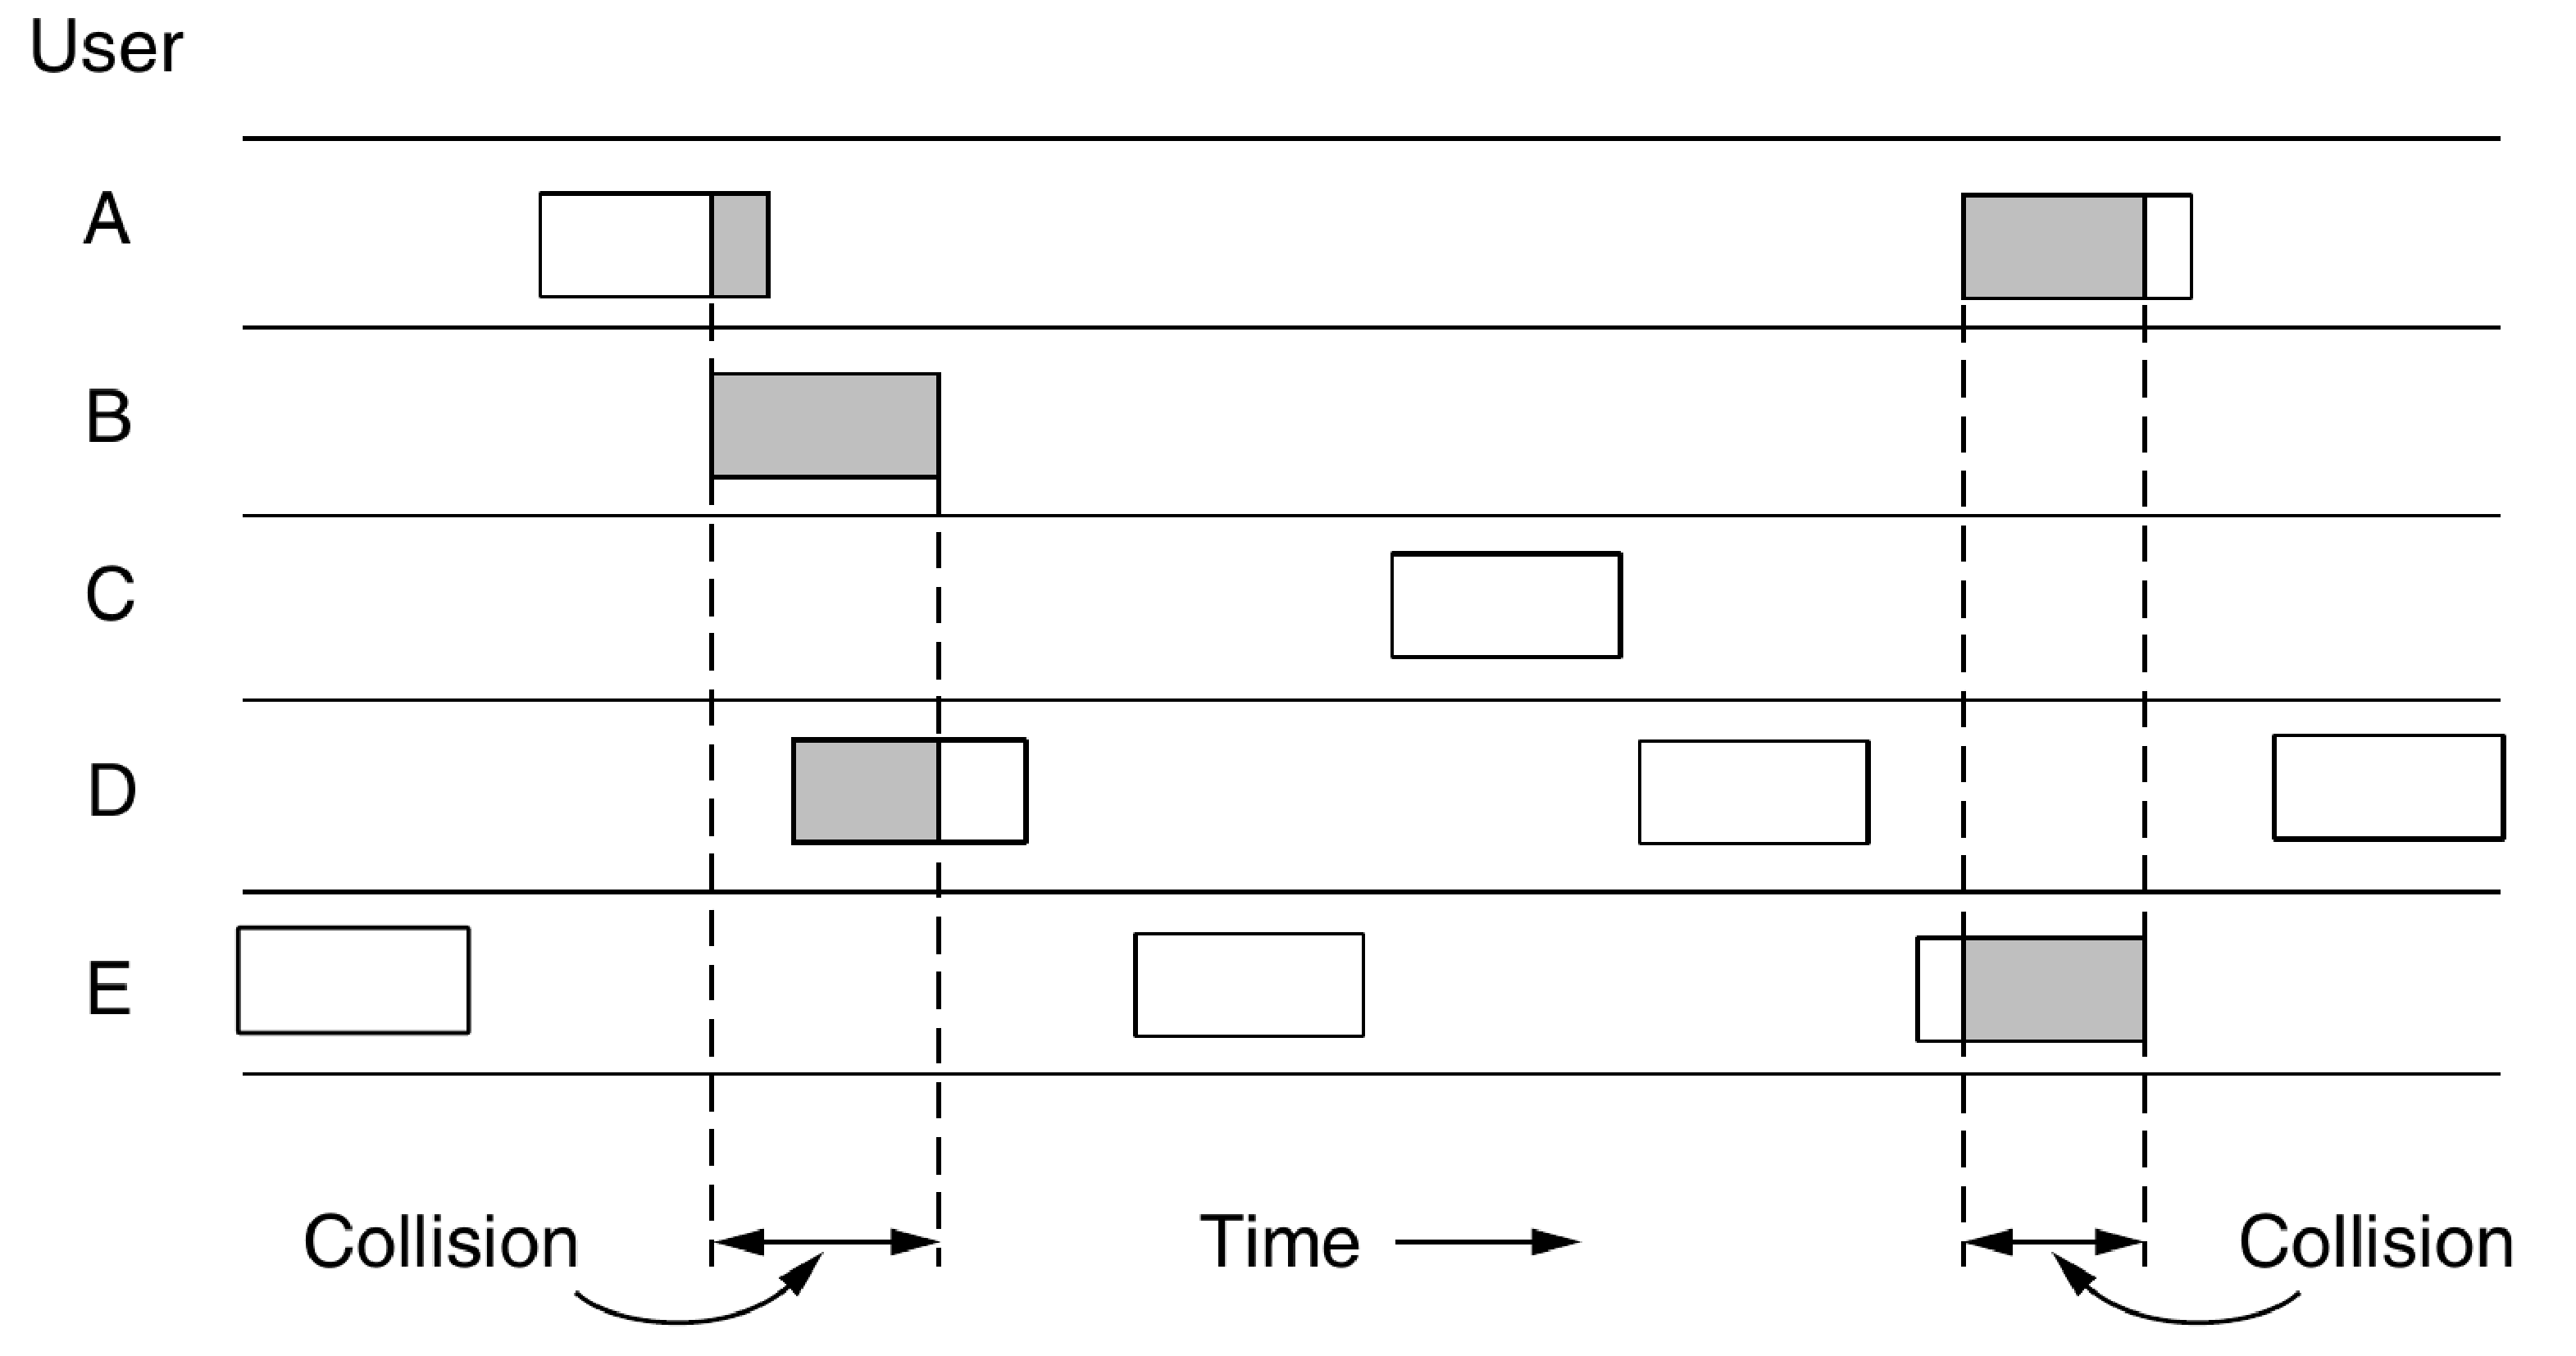
\includegraphics[width=0.7\columnwidth]{figs/fig04-01}
		\end{center}
	\end{figure}
	
\end{frame}

\begin{frame}
	\frametitle{Desempenho do Aloha}

	\begin{itemize}
		\item Desempenho depende da carga do sistema
		\begin{itemize}
			\item Quanto mais usuários tentam enviar informação, mais colisões ocorrem e maior a banda desperdiçada em colisões.
			\item Vazão média como função da carga oferecida ao sistema.
		\end{itemize}
		\item Para baixas cargas:
		\begin{itemize}
			\item Baixa probabilidade de colisão.
			\item Baixa vazão (pouco tráfego), comparável à alocação estática.
			\item Atrasos muito menores (transmissão pode ocorrer logo).
		\end{itemize}
		\item Para altas cargas
		\begin{itemize}
			\item Grande número de colisões.
			\item Baixa vazão (menor que a alocação estática).
		\end{itemize}
		\item Desempenho em pontos intermediários?
	\end{itemize}
\end{frame}

\begin{frame}
	\frametitle{Desempenho do Aloha}

	\begin{itemize}
		\item ``Tempo de quadro'': tempo necessário para transmitir um quadro de tamanho fixo (tamanho do quadro dividido pela taxa).
		\item Geração de novos quadros:
		\begin{itemize}                            
			\item Segue distribuição de Poisson com média de $N$ quadros por tempo de quadro.
		\end{itemize}
		\item Se $N>1$,  então a taxa de geração de quadros é maior do que o canal consegue suportar e praticamente todo quadro sofrerá colisão.
		\item Para vazão razoãvel: $0 < N < 1$.
		\item Colisões geram retransmissões.
		\item Quadros novos e antigos modelados por distribuição de Poisson com média de $G$ quadros por tempo de quadro.
		\item Para baixa carga $G \approx N$ e para alta carga $G > N$.
		\item Vazão: $S = GP_0$,  onde $P_0$ é a probabilidade de o quadro não sofrer colisão.
	\end{itemize}
\end{frame}

\begin{frame}
	\frametitle{Desempenho do Aloha}

	\begin{itemize}
		\item Probabilidade de sucesso:
		\begin{itemize}
		    \item Não pode haver outra transmissão durante o tempo do quadro
		    \item Intervalo de contenção: duas vezes o tempo do quadro
		    \item Probabilidade de que nenhum outro quadro comece durante o intervalo de contenção
		\end{itemize}
	\end{itemize}
	
	\begin{columns}
		\column{0.4\linewidth}
		\begin{small}
		\begin{align*}
		    \mathrm{Pr}[k] &= \frac{G^k e^{-G}}{k!} \\ \\
		    P_0 &= \frac{(2G)^0 e^{-2G}}{0!} = e^{-2G} \\		    
		\end{align*}
		\end{small}
		
		\column{0.6\linewidth}
		\begin{figure}[t]
			\begin{center}
				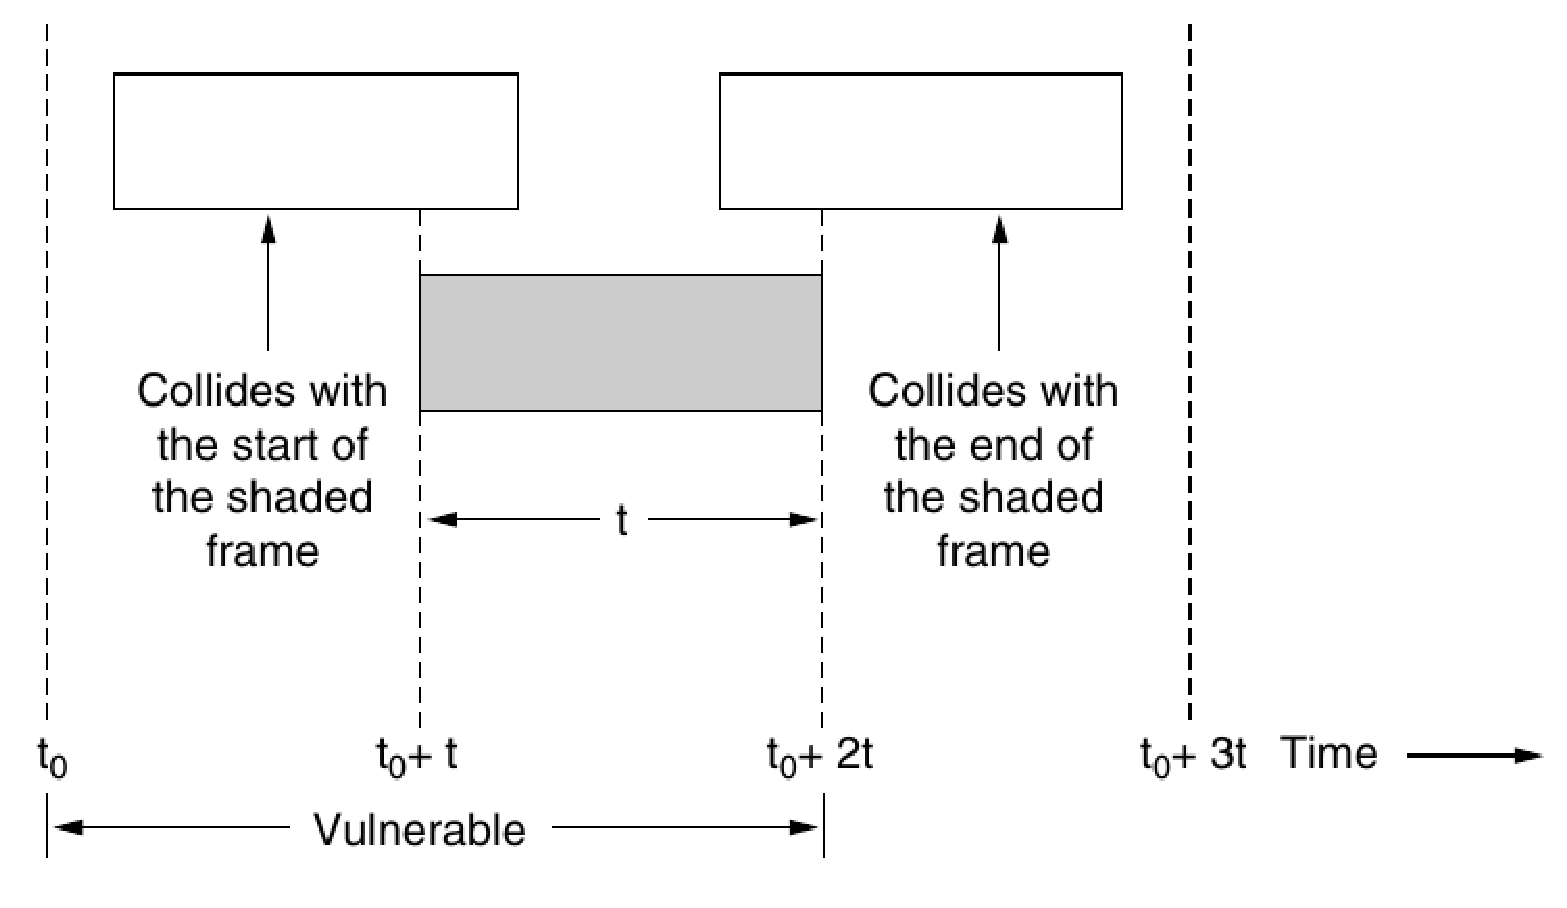
\includegraphics[width=0.9\columnwidth]{figs/fig04-02}
			\end{center}
		\end{figure}
	\end{columns}
\end{frame}

\begin{frame}
	\frametitle{Desempenho do Aloha}

	\begin{itemize}
		\item Portanto: $S = GP_0 = Ge^{-2G}$
		\begin{figure}[t]
			\begin{center}
				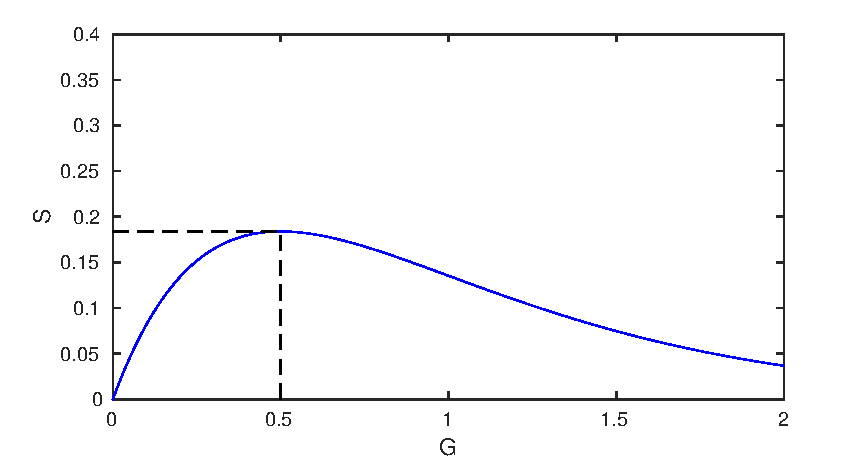
\includegraphics[width=0.55\columnwidth]{figs/aloha-cap}
			\end{center}
		\end{figure}
		\item Ponto de máxima vazão:
		\begin{equation*}
		    \frac{dS}{dG} = \frac{d}{dG} Ge^{-2G} = e^{-2G} - 2Ge^{-2G} = 0
		\end{equation*}
		\item Resolvendo: $G^* = 0,5$ e $S^* = 1/(2e) = 0,184$
	\end{itemize}
	
\end{frame}

\begin{frame}
	\frametitle{Slotted Aloha}
	
	\begin{itemize}
		\item Mudança de tempo contínuo para tempo discreto
		\item Eixo temporal: sequência de slots de tempo $T$, dentro do qual pode ser enviado um quadro
		\item Sincronismo dos transmissores
		\item Se um quadro é gerado durante um slot, ele é enfileirado até o início do próximo slot
		\item Contenção só ocorre entre quadros gerados durante o mesmo slot
		\item Período de contenção reduzido de 2 para 1 tempo de quadro
	\end{itemize}
	
	\begin{columns}
		\column{0.35\linewidth}
		\begin{small}
		\begin{align*}
		    P_0 &= e^{-G} \\
		    S &= Ge^{-G} \\
		    \text{Máximo: }& \begin{cases} S^* = 0,368 \\ G^* = 1 \end{cases}
		\end{align*}
		\end{small}		
		\column{0.65\linewidth}\vspace{-0.3cm}
		\begin{figure}[t]
			\begin{center}
				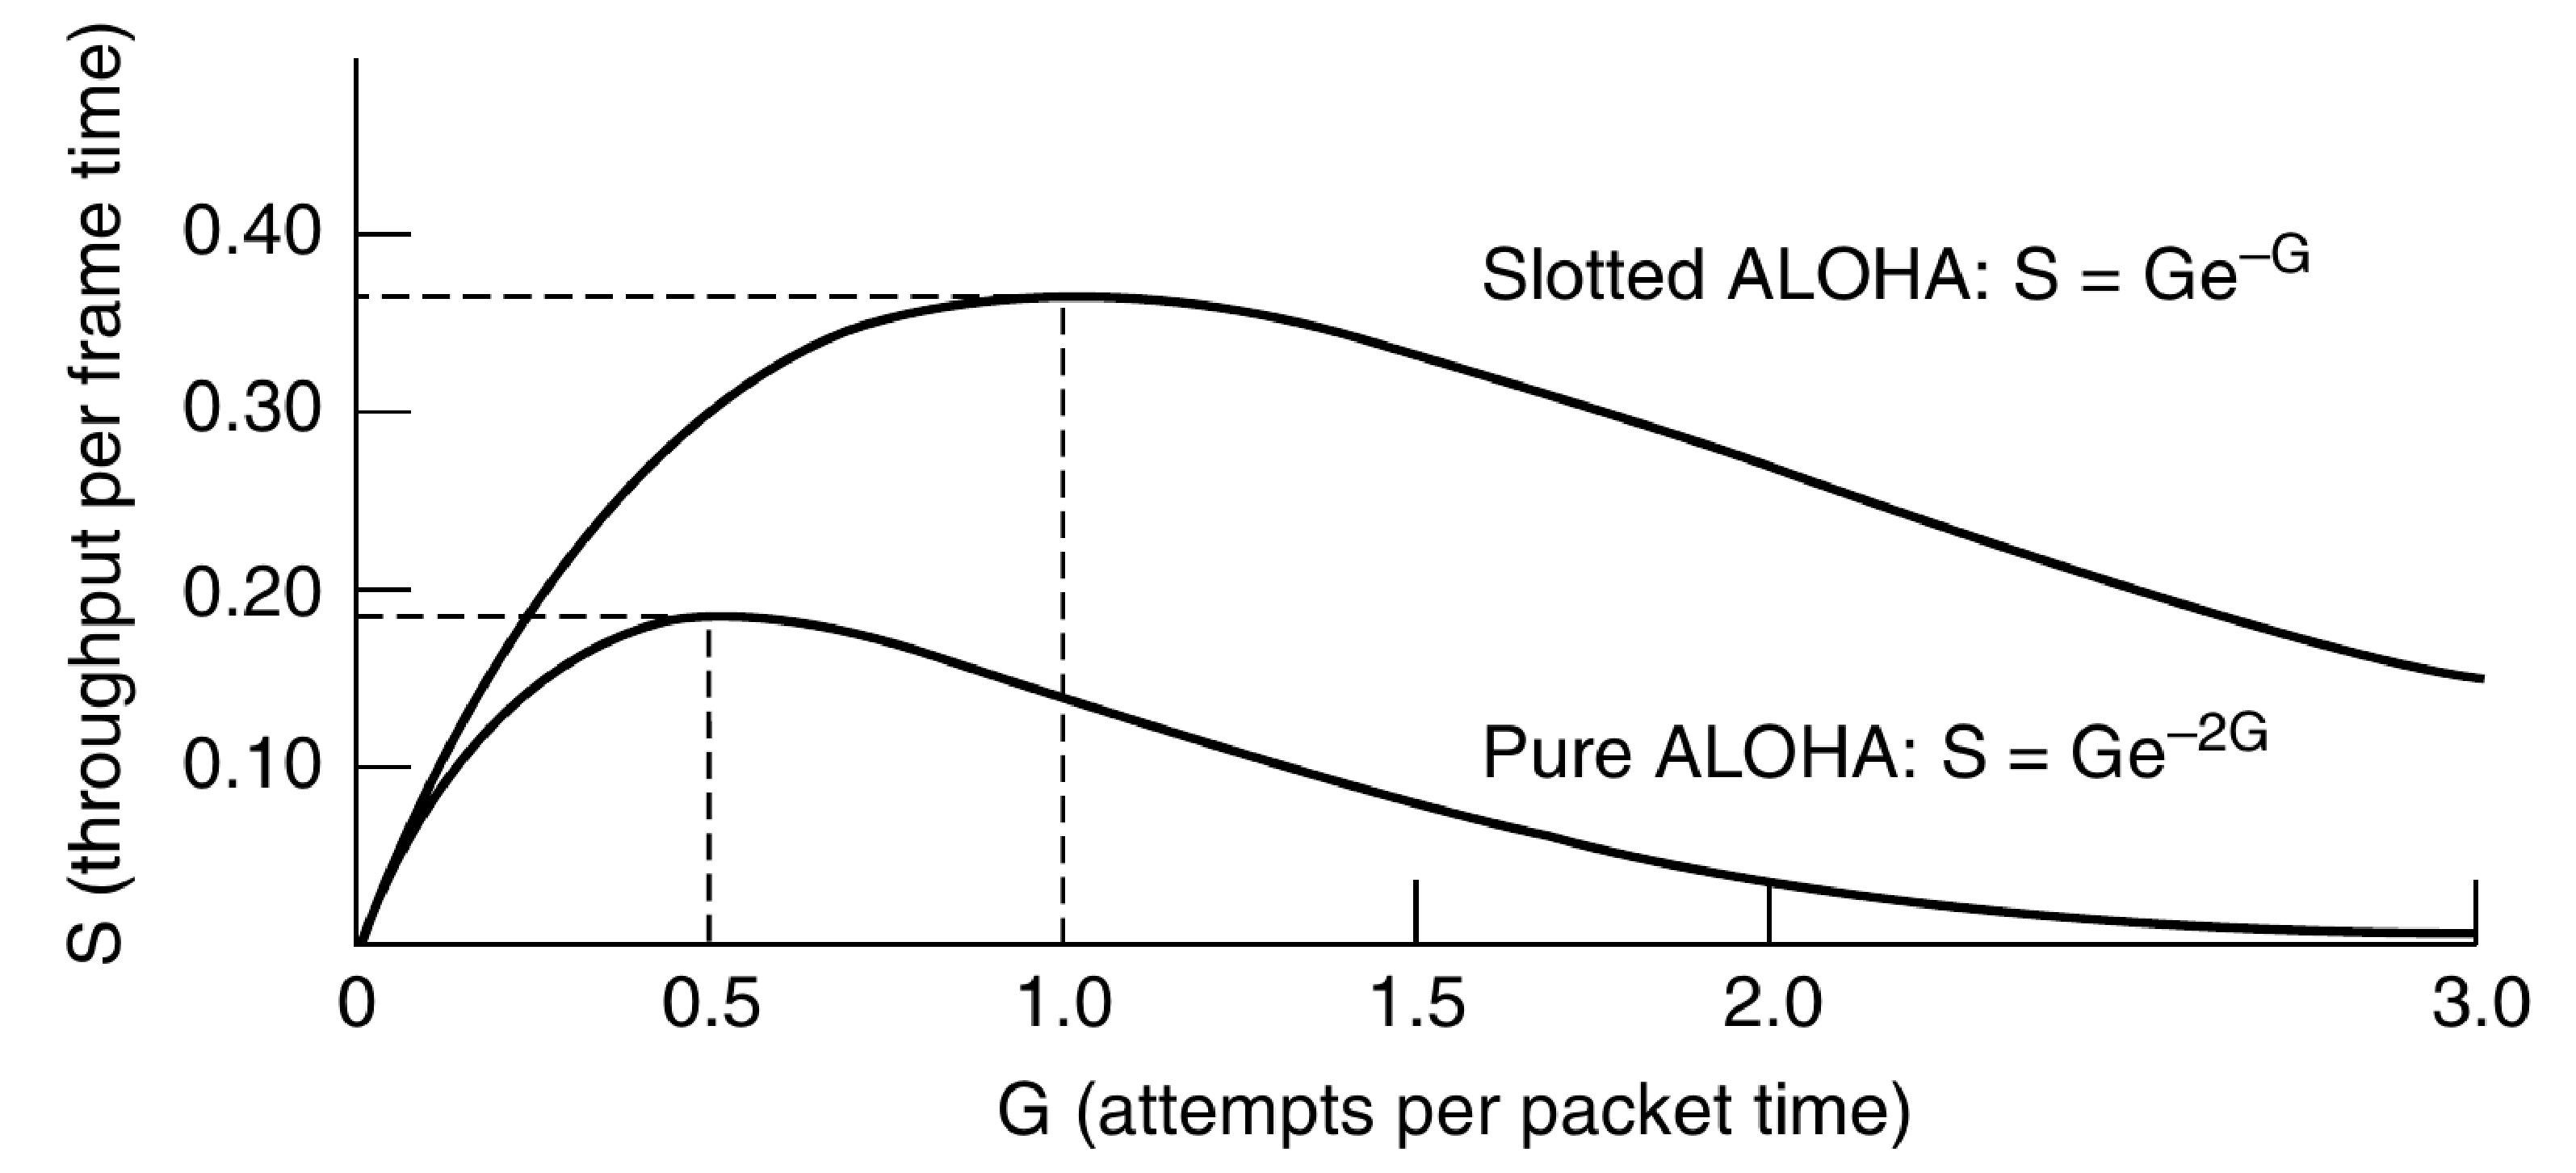
\includegraphics[width=\columnwidth]{figs/fig04-03}
			\end{center}
		\end{figure}
	\end{columns}
\end{frame}

\begin{frame}
	\frametitle{CSMA}
	
	\begin{itemize}
		\item \textbf{Aloha}: colisões são informadas após sua ocorrência
		\item \textbf{Carrier sensing}: capacidade de detectar que outros nós estão transmitindo após um pequeno atraso de propagação
		\item Não há sentindo em transmitir quando se detecta previamente uma colisão
		\item \textbf{Protocolos CSMA}:
		\begin{itemize}
		    \item Carrier Sense Multiple Access
		    \item Variações quanto à persistência
		    \item Transmissão só ocorre se canal for detectado como desocupado
		\end{itemize}
		\item \textbf{Colisões}: ocorrem somente quando dois usuários começam a transmitir muito próximo um do outro, de forma que não haja tempo de realizar a detecção
	\end{itemize}
	
\end{frame}

\begin{frame}
	\frametitle{CSMA}
	
	\begin{itemize}
		\setlength{\leftmarginii}{0.8cm}
		\item CSMA persistente:		
		\begin{itemize}		    
		    \item[1)] Se o canal estiver desocupado, transmita.
		    \item[2)] Se o canal estiver ocupado, espere desocupar e transmita.
		    \item[3)] Em caso de colisão, espere um tempo aleatório e volte para 1.
		\end{itemize}
		\item Outras variações do CSMA modificam os 2 primeiros passos
		\item Não-persistente:
		\begin{itemize}
		    \item[1)] Se o canal estiver desocupado, transmita.
		    \item[2)] Se o canal estiver ocupado, espere um tempo aleatório e volte para 1.
		\end{itemize}
		\item $p$ – persistente: (sistema com slots)
		\begin{itemize}
		    \item[1)] Se o canal estiver desocupado, transmita com probabilidade $p$. Espere um slot com probabilidade $1 - p$, repita passo 1.
		    \item[2)] Se o canal estiver ocupado, espere desocupar e volte para 1.
		\end{itemize}
	\end{itemize}
	
\end{frame}

\begin{frame}
	\frametitle{CSMA}
	
	\begin{itemize}		
		\item CSMA persistente:
		\begin{itemize}
		    \item Se múltiplas estações estão esperando o canal ficar desocupado, haverá colisão
		    \item Não-persistente ou p-persistente reduz essa probabilidade de colisão, às custas de maiores atrasos
		\end{itemize}\vspace{0.4cm}
		\item Parâmetro de desempenho:
		\begin{itemize}
		    \item Tempo máximo entre um nó começar a transmitir e outro nó ser capaz de detectar essa transmissão
		    \item Depende de: atraso de propagação e atraso de deteção
		    \item Queda de desempenho em caso de aumento desses atrasos
		\end{itemize}
	\end{itemize}
	
\end{frame}

\begin{frame}
	\frametitle{Desempenho dos algoritmos}
	
	\begin{figure}[t]
		\begin{center}
			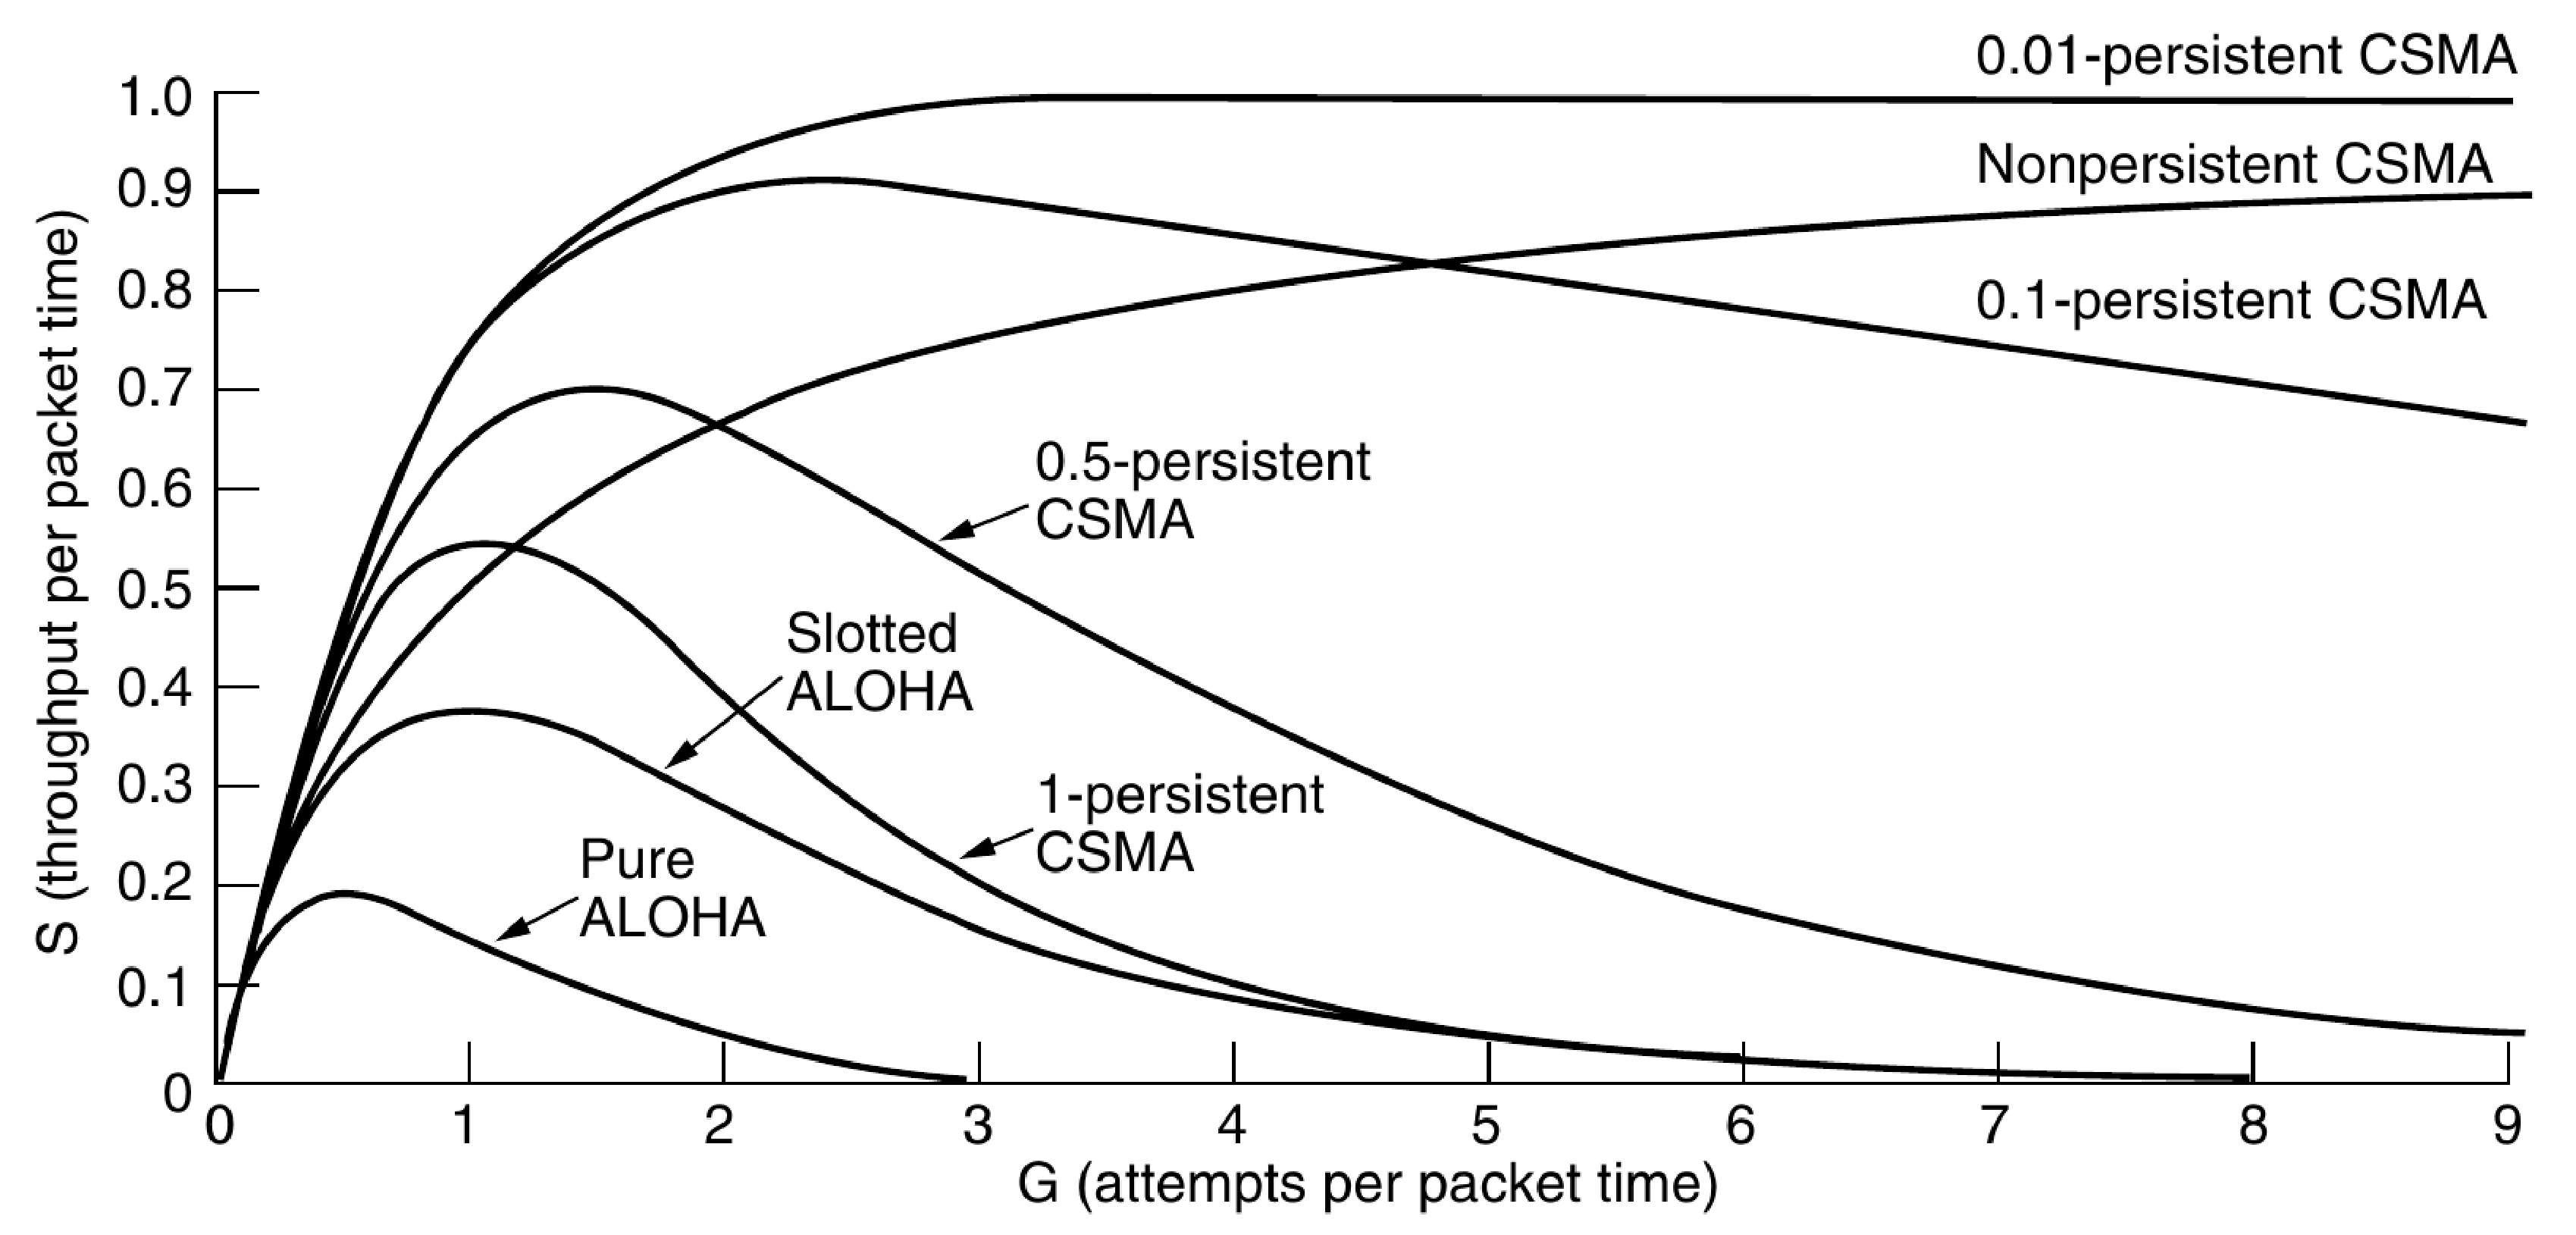
\includegraphics[width=0.95\columnwidth]{figs/fig04-04}
		\end{center}
	\end{figure}
	
\end{frame}

\begin{frame}
	\frametitle{CSMA}
	
	\begin{itemize}
	    \item Claramente, CSMA é melhor que o Aloha.
	    \item Como escolher a persistência?
	    \begin{itemize}
		\item Depende da carga oferecida em que se deseja operar, e 
		\item Também depende do atraso médio desejado.
	    \end{itemize}
	    \item Todos esses esquemas aleatórios possuem um atraso menor do que o TDMA até que se aproximem do seu limite de vazão.
	    \item Quanto maior a carga total $G(n)$ no ponto de operação, maior o atraso.
	    \item 1 – Persistente resulta na melhor característica de atraso para um mesmo $G(n)$.
	\end{itemize}
	
\end{frame}

\begin{frame}
	\frametitle{CSMA/CD}
	
	\begin{itemize}
	    \item Em algumas situações, os nós podem ouvir uns aos outros mesmo quando estão transmitindo. (ex. barramento compartilhado)
	    \item Em caso de colisão, todos os nós a detectam em um máximo atraso de propagação $2\tau$.
	    \item Se o nó sabe que está ocorrendo colisão, ele pode parar de transmitir para minimizar a quantidade de tempo perdida na colisão
	    \item Essa modificação do CSMA é conhecida como CSMA/CD (CSMA com deteção de colisão)
	    \item No CSMA/CD as colisões são detectadas antes que o pacote inteiro seja transmitido.
	    \item Uma vez que um nó começa a transmitir, quanto tempo leva até que ele saiba que ocorreu uma colisão?
	\end{itemize}
	
\end{frame}

\begin{frame}
	\frametitle{CSMA/CD}
	
	\begin{itemize}
	    \item Detecção de colisão
	    \begin{figure}[t]
		\begin{center}
			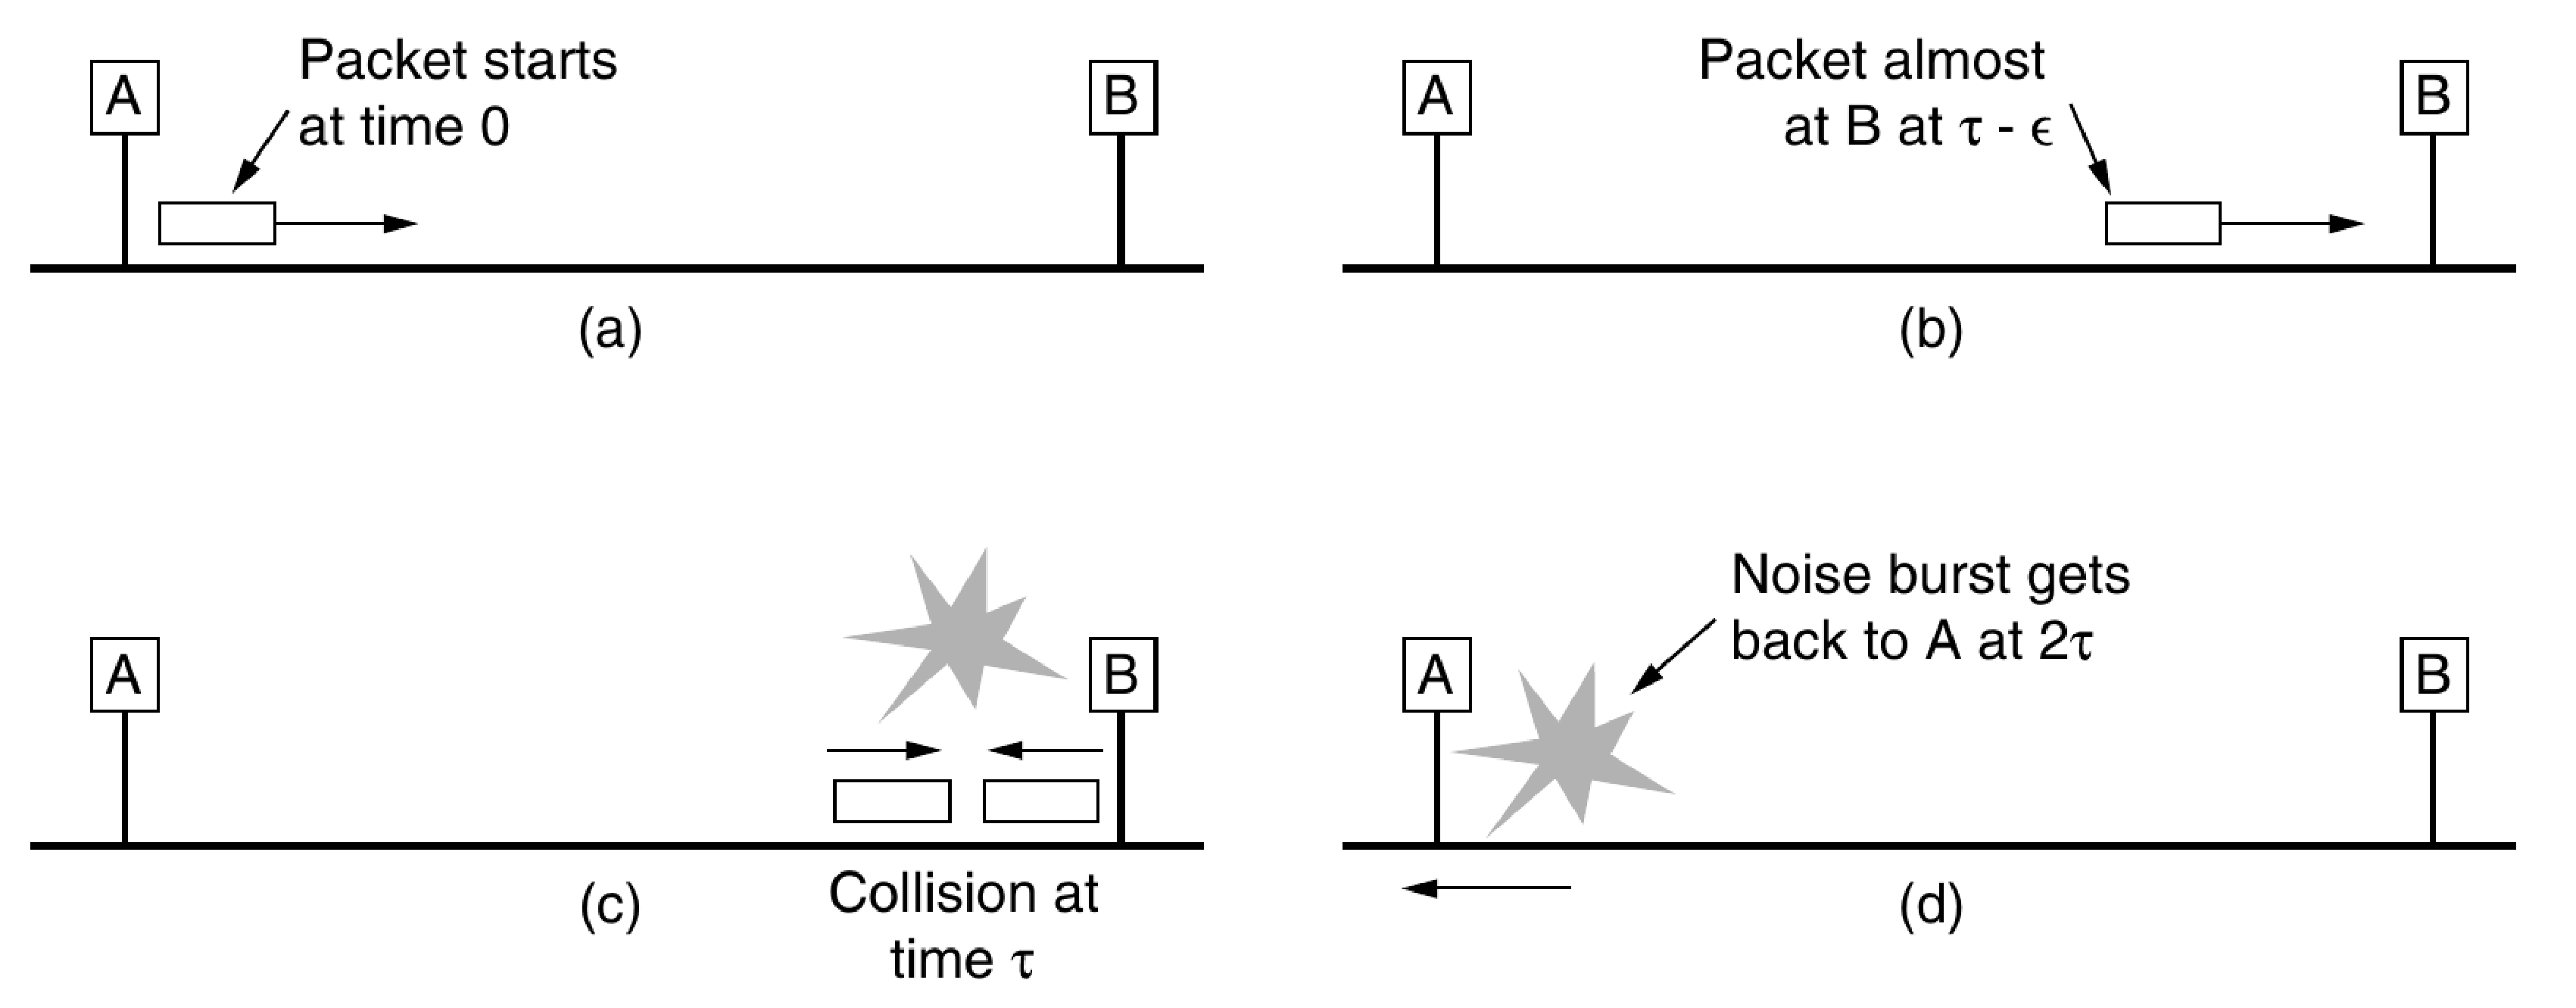
\includegraphics[width=0.7\columnwidth]{figs/fig04-15}
		\end{center}
	    \end{figure}
	    \item Estados do CSMA/CD
	    \begin{figure}[t]
		\begin{center}
			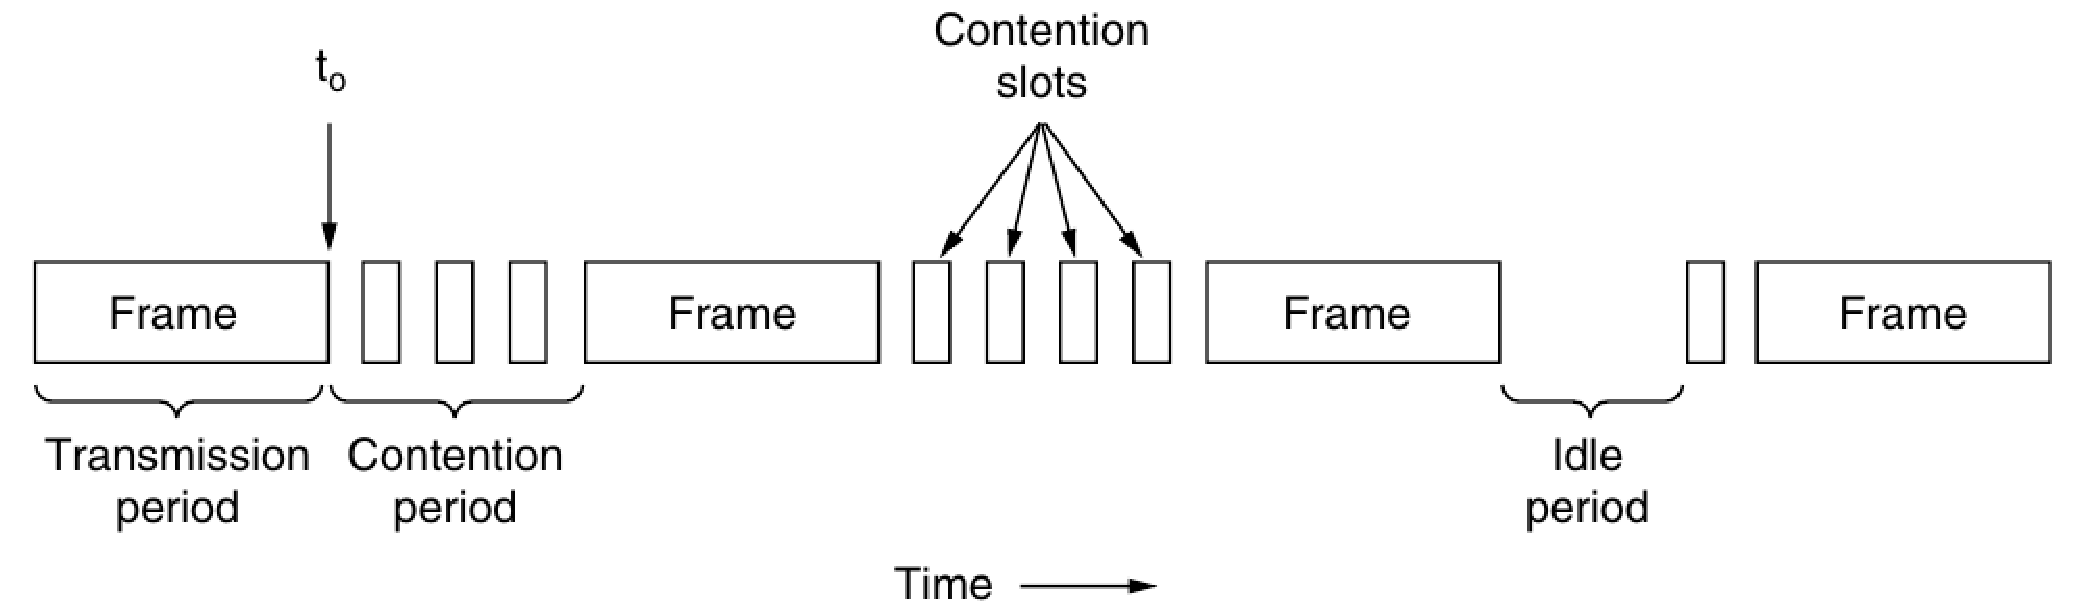
\includegraphics[width=0.6\columnwidth]{figs/fig04-05}
		\end{center}
	    \end{figure}
	\end{itemize}
	
\end{frame}
